\documentclass{article}

% \usepackage[preprint]{neurips_2026}
\usepackage{neurips_2026}
\usepackage[utf8]{inputenc} % allow utf-8 input
\usepackage[T1]{fontenc}    % use 8-bit T1 fonts
\usepackage{hyperref}       % hyperlinks
\usepackage{url}            % simple URL typesetting
\usepackage{booktabs}       % professional-quality tables
\usepackage{amsfonts}       % blackboard math symbols
\usepackage{nicefrac}       % compact symbols for 1/2, etc.
\usepackage{microtype}      % microtypography
\usepackage{xcolor}         % colors

\usepackage{graphicx}
\usepackage[strings]{underscore} % 自动处理文本中的下划线
\usepackage{grffile}           % 增强文件名处理，允许更多特殊字符
\usepackage{amsmath}
\usepackage{amssymb}
\usepackage{amsthm}
\usepackage{multirow}
\usepackage{wrapfig}
\newtheorem{proposition}{Proposition}
\newcommand{\don}[1]{\textcolor{blue}{[Dongfang: #1]}}

\title{When Adapter Training Hurts: Manifold Preservation for Vector Retrieval}

\author{%
  Dongfang Zhao \\
  Tacoma School of Engineering and Technology\\
  Paul G. Allen School of Computer Science \& Engineering\\
  University of Washington\\
  \texttt{dzhao@cs.washington.edu} \\
}

\begin{document}

\maketitle

\begin{abstract}
We study how lightweight adapters trained on top of frozen vision-language
encoders behave under distribution shift, and identify a
structural in-distribution/out-of-distribution (ID/OOD) tradeoff among
existing adapter training paradigms. Global contrastive objectives such as
ICon and SRL, when paired with high-capacity adapters, achieve near-perfect
in-distribution Label Precision on CIFAR-100 ($0.999$ and $0.992$ at $K=1$,
$\text{nprobe}=1$) but collapse to $0.557$ and $0.520$ on the unseen classes
of Food-101: a $44$--$47$ percentage point inversion between the two
scenarios. Low-capacity alternatives such as LoRA avoid this collapse but
underperform substantially in-distribution. We propose \textbf{Euclidean
Geodesic Alignment (EGA)}, a residual adapter trained with a small-margin
triplet loss on the class-aware neighborhood graph of pre-trained embeddings.
EGA converges to a sparse-gradient scheme in which $96.5\%$ of training
triplets produce zero gradient at steady state, preserving the pre-trained
semantic structure for unseen categories while still permitting high-capacity
in-distribution refinement. Across CIFAR-100 (ID) and three OOD benchmarks
(CIFAR-10, FGVC-Aircraft, Food-101), the six methods we evaluate trace out a
Pareto frontier in the (ID, OOD) Label Precision plane, and EGA is the only
adapter that is not strictly dominated: methods that exceed EGA's
in-distribution precision (ICon, SRL) collapse on OOD; methods that match
EGA on OOD (LoRA, frozen baseline) underperform in-distribution.
\end{abstract}

\section{Introduction}

Modern retrieval systems increasingly rely on embedding models such as CLIP~\cite{clip_icml21} for their remarkable zero-shot semantic capabilities. These models provide highly generalizable latent spaces that serve as excellent starting points for vector similarity search. However, when deploying these systems to specialized domains, practitioners often seek to further align the embeddings with domain-specific category structures to maximize retrieval accuracy. Because full-scale fine-tuning is computationally prohibitive and risks destroying the foundational zero-shot knowledge, parameter-efficient adaptation has emerged as the standard paradigm: lightweight adapters are trained on a labeled subset of the target task while the massive pre-trained backbone remains frozen.

A subtle but consequential aspect of this paradigm is that retrieval systems do not only serve queries from the categories seen during adapter training. In real deployments, the database and the query stream routinely contain \emph{unseen} categories that were absent from the labeled subset, and the adapter must continue to support meaningful retrieval over these. The standard practice is training adapters with global contrastive objectives such as ICon~\cite{alshammariunifying} and SRL~\cite{dong2025improve} that compute losses over the full pairwise similarity matrix in each mini-batch; however, this approach optimizes aggressively for the seen-class structure with no explicit mechanism to preserve the embedding geometry of unseen categories.

We show that this paradigm produces a structural in-distribution/out-of-distribution (ID/OOD) tradeoff rather than a uniformly improved adapter. On in-distribution data (CIFAR-100), high-capacity global contrastive adapters reach Label Precision near $1.0$: ICon at $0.999$, SRL at $0.992$ at $K=1$, $\text{nprobe}=1$. On the strictly unseen classes of Food-101, the same adapters collapse to $0.557$ and $0.520$, dropping $44$ and $47$ percentage points below their own in-distribution scores and $32$ to $36$ percentage points below the \emph{frozen} CLIP baseline. Restricting capacity through low-rank adapters such as LoRA~\cite{hu2022lora} avoids this catastrophic collapse but pays a different cost: LoRA's in-distribution Label Precision is bounded around $0.61$--$0.67$, far below what high-capacity adapters can achieve when overfitting is not punished by distribution shift.

We propose Euclidean Geodesic Alignment (EGA), a manifold-preserving adapter that occupies a Pareto-optimal balance between these schemes. EGA combines three design choices: (i) a zero-initialized residual structure, (ii) an $\ell_2$ normalization constraint, and (iii) a small-margin triplet loss on the class-aware neighborhood graph. The triplet loss with small margin produces a self-limiting optimization dynamic: as the adapter converges on seen classes, the fraction of triplets violating the margin decays rapidly, and at steady state $96.5\%$ of training triplets contribute zero gradient. The high-capacity architecture is therefore allowed to tightly refine the regions of the embedding space that the seen classes occupy, while remaining largely inactive over the rest, which is a property that protects the pre-trained semantic structure of unseen categories from the dense global reshaping that drives ICon and SRL to OOD failure.

We evaluate EGA on CIFAR-100 (in-distribution) and three OOD benchmarks (CIFAR-10, FGVC-Aircraft, Food-101), comparing against the frozen CLIP baseline, global contrastive adapters (ICon, SRL), and two LoRA configurations (LoRA+InfoNCE, LoRA+Triplet). The six methods trace out a Pareto frontier in the (ID, OOD) Label Precision plane, and EGA is the only adapter that is not strictly dominated by any other: it reaches $0.851$ in-distribution Label Precision (within $15$ percentage points of the ICon/SRL ceiling), while improving over the frozen baseline on Aircraft ($+3.6$ pp) and CIFAR-10 ($+0.6$ pp) and bounding the degradation on Food-101 ($-8.3$ pp, versus $-32$ to $-36$ pp for ICon and SRL).

% \paragraph{Contributions}
% This paper makes the following contributions:
% \begin{itemize}
%     \item \textbf{Phenomenon.} We identify a structural ID/OOD tradeoff among existing adapter training paradigms: high-capacity adapters trained with global contrastive objectives achieve near-perfect in-distribution Label Precision but collapse below the frozen baseline on unseen categories, while low-capacity adapters such as LoRA avoid the collapse at the cost of substantial in-distribution underperformance.
%     \item \textbf{Method.} We propose EGA, a manifold-preserving residual adapter trained with a small-margin triplet loss whose self-limiting gradient dynamics permit high-capacity in-distribution refinement while leaving most of the embedding space structurally unmodified.
%     \item \textbf{Evaluation.} Across CIFAR-100 and three OOD benchmarks (CIFAR-10, FGVC-Aircraft, Food-101), EGA is the only adapter on the Pareto frontier of (ID, OOD) Label Precision: no other method we evaluate achieves both EGA's in-distribution refinement and its OOD stability simultaneously.
% \end{itemize}

\section{Related Work}
\label{sec:lit}

\paragraph{Manifold Preservation under Adapter Tuning}
Foundation models such as CLIP~\cite{clip_icml21} produce embedding spaces whose structure encodes both seen class semantics and a broader prior over visual concepts not observed during downstream training. Catastrophic forgetting has been studied extensively in continual and incremental learning settings~\cite{lanza2026degradationfeaturespacecontinual, xue2025protocol}. Recent work has documented analogous degradation phenomena specific to contrastive representations: anisotropic collapse into narrow conic regions~\cite{zhao-etal-2024-representation, gao-etal-2021-simcse}, structural fracturing under modality gap~\cite{10656738, eslami2025mitigate}, and loss of compositional structure under aggressive optimization~\cite{pal2025compositional, savietto2026geometryrepresentationalfailuresvision, 11093676}. To counter these degradations, recent adaptation strategies impose explicit geometric constraints such as orthogonality regularization~\cite{ricci2026boldsymbollambdaorthogonality} or restrict optimization to limited subspaces. EGA leverages the inherent sparsity of triplet loss optimization to confine adapter updates to local neighborhoods of seen classes, leaving the unseen class regions of the pretrained manifold structurally unmodified.

\paragraph{Global Contrastive Objectives and Structural Regularization}
Recent advancements in representation learning often rely on global contrastive objectives to optimize the latent space~\cite{sui2026unicon, koromilas2025principledframeworkmultiviewcontrastive}. A common paradigm involves jointly enforcing alignment for positive pairs and uniformity for the overall feature distribution~\cite{10.5555/3524938.3525859}, a strategy applied across various domains including graph encoders~\cite{10.1609/aaai.v38i14.29479} and multimodal recommendation systems~\cite{zhou2025cm3calibratingmultimodalrecommendation}. While pushing embeddings toward a uniform distribution enhances robustness to background noise~\cite{wu2026pca}, it inherently assumes that all latent regions require the same degree of global scattering. To further refine complex distributions, structural regularization techniques introduce auxiliary constraints. For instance, methods like ICon formulate a unifying framework to systematically align multi view representations~\cite{alshammariunifying}, while geometric constraints are leveraged to improve imbalanced regression tasks~\cite{dong2025improve}. Other approaches attempt to decouple the learning objectives~\cite{kim2025decoupledcontrastivelearningfederated} or apply information theoretic regularizers~\cite{Zhang_2025_ICCV} to control the density of the learned representations. Furthermore, region based distillation techniques have been proposed to enhance fine grained understanding~\cite{jing2024fineclip}. EGA replaces dense global optimization with sparse local triplet updates, preserving out of distribution semantic structure.

\paragraph{Parameter-Efficient Manifold Adaptation}
Parameter efficient adaptation emerged as a standard to prevent catastrophic forgetting and reduce computational overhead when transferring large foundation models~\cite{pmlr-v97-houlsby19a, hu2022lora}. This paradigm has extensively shifted towards vision language models, dominating recent literature due to the prohibitive cost of full scale fine tuning~\cite{lin2025visionlanguagemodelssurvey}. Methods such as Visual Prompt Tuning~\cite{10.1007/978-3-031-19827-4_41} and Tip Adapter demonstrate that lightweight tuning can effectively specialize representations for downstream tasks without altering the frozen backbone~\cite{10.1007/978-3-031-19833-5_29}. Furthermore, extensive benchmarking confirms that parameter efficient techniques can rival full fine tuning while preserving the generalizable representations of the foundation model~\cite{sharma2025benchmarking}. To further protect the pre trained manifold during initial training steps, zero initialization strategies have proven highly effective. For instance, conditional control mechanisms in image generation initialize adapter weights to zero, ensuring the model behaves exactly like the frozen base model before any optimization occurs~\cite{10377881}. EGA integrates a zero initialized residual adapter with a localized geometric objective, achieving both parameter efficiency and targeted manifold smoothing.

\paragraph{Vector Similarity Search and Metric Consistency}
Vector similarity search is the foundational engine for retrieving high dimensional representations at scale. The systems community has developed highly optimized indexing algorithms to handle billion scale datasets. Foundational works such as FAISS leverage hardware acceleration for fast similarity search~\cite{johnson2019billion}, and Hierarchical Navigable Small World graphs establish the core topology for efficient approximate retrieval~\cite{malkov2018efficient}. Meanwhile, hybrid structures like DiskANN and SPANN achieve exceptional speed by efficiently managing memory and disk hierarchies~\cite{subramanya2019diskann, chen2021spann}. Recent advancements continue to refine these topologies, exploring crossing sparse proximity graphs~\cite{NEURIPS2024_bab1486c} and analyzing the theoretical constructions of navigable graphs for high dimensional nearest neighbor search~\cite{NEURIPS2024_6dc63b40}. Furthermore, system level studies optimize retrieval latency and stability by aligning best first search algorithms with solid state drives~\cite{osdi25pipeann} and enabling direct insertions in large scale indices~\cite{fast26odinann}. To reduce the computational cost of exact distance calculations during the retrieval phase, approximation techniques such as low rank matrix factorization have also been introduced to accelerate inner product evaluations~\cite{jaasaari2024lorann}. However, extensive theoretical analyses reveal that popular approximate nearest neighbor implementations still face severe worst case performance limitations~\cite{NEURIPS2023_d0ac28b7}. EGA proactively recalibrates the metric manifold prior to index construction, enabling standard search backends to achieve superior semantic recall without requiring complex algorithmic reengineering.

\section{Methodology}
\label{sec:method}

\subsection{Problem Formulation}
\label{sec:formulation}

Let $\phi : \mathcal{X} \to \mathbb{R}^d$ denote a frozen vision-language encoder
(e.g., CLIP ViT-B/32) that maps an image $x \in \mathcal{X}$ to a unit-normalized
embedding $\mathbf{z} = \phi(x) \in \mathbb{S}^{d-1}$.
We are given a set of labeled training images $\mathcal{D}_\text{train} =
\{(x_i, y_i)\}_{i=1}^{N}$, where $y_i \in \mathcal{Y}_\text{seen}$ belongs to a
set of \emph{seen} classes. At inference time, the retrieval system must operate
over a database that also contains images from a disjoint set of \emph{unseen}
classes $\mathcal{Y}_\text{unseen}$, with
$\mathcal{Y}_\text{seen} \cap \mathcal{Y}_\text{unseen} = \emptyset$.

Our goal is to learn a lightweight adapter
$f_\theta : \mathbb{S}^{d-1} \to \mathbb{S}^{d-1}$
such that the transformed embeddings $\hat{\mathbf{z}} = f_\theta(\mathbf{z})$
support more accurate approximate nearest neighbor (ANN) retrieval on
\emph{both} seen and unseen classes, without access to any unseen-class labels
during training.

\paragraph{Evaluation metrics.}
We evaluate retrieval quality along two complementary dimensions.

Label Precision@$K$ measures the semantic quality of retrieved
results—whether the $K$ nearest neighbors in the transformed space share the
same class label as the query:
\begin{equation}
    \text{LP}@K = \frac{1}{|\mathcal{Q}|} \sum_{q \in \mathcal{Q}}
    \frac{1}{K} \sum_{k=1}^{K}
    \mathbf{1}\!\left[y_{\hat{n}_k(q)} = y_q\right],
    \label{eq:lp}
\end{equation}
where $\mathcal{Q}$ is the query set and $\hat{n}_k(q)$ denotes the $k$-th
nearest neighbor of $q$ in the transformed embedding space.

ANNS Recall@$K$ measures the geometric fidelity of the ANN index—the
fraction of true $K$ nearest neighbors (under exact search) that are recovered
by the approximate index at a given search budget $\text{nprobe}$:
\begin{equation}
    \text{AR}@K = \frac{1}{|\mathcal{Q}|} \sum_{q \in \mathcal{Q}}
    \frac{\left|\mathcal{N}_K^\text{exact}(q)
          \cap \mathcal{N}_K^\text{approx}(q)\right|}{K},
    \label{eq:ar}
\end{equation}
where $\mathcal{N}_K^\text{exact}(q)$ and $\mathcal{N}_K^\text{approx}(q)$
denote the exact and approximate top-$K$ neighbor sets, respectively.

The two metrics capture distinct failure modes: an adapter may improve
$\text{LP}@K$ by tightening within-class clusters (semantic improvement) while
simultaneously improving $\text{AR}@K$ by making the geometry more amenable to
IVF-based indexing (geometric improvement). As we show in
Section~\ref{sec:eval}, global contrastive objectives achieve high
$\text{AR}@K$ on seen classes but collapse on \emph{both} metrics for unseen
classes, whereas EGA improves both simultaneously under the OOD setting.

\subsection{Manifold-Preserving Adapter Design}
\label{sec:design}

EGA introduces a lightweight adapter $f_\theta$ composed of stacked residual
blocks with a final refinement layer. The architecture is deliberately
constrained by three design principles, each of which serves a distinct role
in preserving the pretrained manifold.

\paragraph{Residual connection with zero initialization.}
Each EGA block applies a residual update of the form
\begin{equation}
    \mathbf{z}' = \mathbf{z} + g_\theta(\mathbf{z}),
    \label{eq:residual}
\end{equation}
where $g_\theta$ is a learned transformation initialized so that
$g_\theta(\mathbf{z}) \approx \mathbf{0}$ at the start of training.
Concretely, the final linear layer of $g_\theta$ is initialized to zero,
making $f_\theta$ an identity mapping at initialization.
This guarantees that training begins from the pretrained geometry rather
than a random perturbation, and that the adapter can only \emph{refine}
rather than replace the CLIP embedding.
As confirmed by our ablation (Table~\ref{tab:ablation}), removing the
residual connection causes accuracy to collapse from $0.70$ to $0.01$,
because the lightweight MLP cannot reconstruct complex semantic relationships
from seen-class data alone.

\paragraph{Feature gating.}
Inside each residual block, the transformed signal passes through a
feature-gating module:
\begin{equation}
    \text{Gate}(\mathbf{h}) = \mathbf{h} \odot \sigma\!\left(
        W_2\, \text{GELU}(W_1 \mathbf{h})
    \right),
    \label{eq:gate}
\end{equation}
where $W_1 \in \mathbb{R}^{(d/4) \times d}$, $W_2 \in \mathbb{R}^{d \times (d/4)}$,
$\sigma$ is the sigmoid function, and $\odot$ denotes elementwise
multiplication. This structure, analogous to Squeeze-and-Excitation
networks~\cite{hu2018squeeze}, learns a per-dimension importance weight that
amplifies retrieval-relevant dimensions and suppresses noisy ones.
The bottleneck ratio of $1/4$ is chosen to prevent the gating network from
overfitting on seen-class data, as validated in Table~\ref{tab:sensitivity}.

\paragraph{$\ell_2$ normalization.}
The final output of $f_\theta$ is projected back onto the unit hypersphere
$\mathbb{S}^{d-1}$ via $\ell_2$ normalization:
\begin{equation}
    \hat{\mathbf{z}} = \frac{f_\theta(\mathbf{z})}
                            {\|f_\theta(\mathbf{z})\|_2}.
    \label{eq:l2norm}
\end{equation}
This constraint ensures that the transformed embeddings remain in the same
metric space as the original CLIP embeddings, so that Euclidean distance
and cosine similarity remain interchangeable on the hypersphere.
Removing this constraint degrades retrieval performance by $4.2$ percentage
points (Table~\ref{tab:ablation}), confirming that hypersphere consistency
is necessary for stable ANN indexing.

\paragraph{Full forward pass.}
Let $\text{Block}_i$ denote the $i$-th EGA block consisting of a two-layer
MLP with LayerNorm followed by feature gating, and let $\text{Refine}$
denote the final linear projection with LayerNorm. The complete forward pass
for an input embedding $\mathbf{z} \in \mathbb{S}^{d-1}$ is:
\begin{equation}
    \hat{\mathbf{z}} = \ell_2\!\left(
        \text{Refine}\!\left(
            \text{Block}_2\!\left(
                \text{Block}_1(\mathbf{z})
            \right)
        \right)
    \right).
    \label{eq:forward}
\end{equation}
The total number of trainable parameters is approximately $4.2M$ for
$d = 512$ and hidden dimension $2048$, which is negligible compared to
the frozen CLIP backbone ($\sim$150M parameters).

\subsection{Local Triplet Training and Gradient Sparsity}
\label{sec:training}

\paragraph{Training objective.}
Given a mini-batch sampled from $\mathcal{D}_{\text{train}}$, we construct
triplets $(a, p, n)$ where $a$ is an anchor image, $p$ is a positive sampled
uniformly from the same class as $a$, and $n$ is a negative sampled uniformly
from a different class. The adapter is trained with the standard triplet
margin loss:
\begin{equation}
    \mathcal{L} = \frac{1}{|\mathcal{B}|}
    \sum_{(a,p,n) \in \mathcal{B}}
    \max\!\left(0,\;
        d\!\left(\hat{\mathbf{z}}_a, \hat{\mathbf{z}}_p\right)
        - d\!\left(\hat{\mathbf{z}}_a, \hat{\mathbf{z}}_n\right)
        + m
    \right),
    \label{eq:triplet}
\end{equation}
where $d(\cdot,\cdot)$ denotes Euclidean distance, $m > 0$ is the margin
hyperparameter, and $\hat{\mathbf{z}} = f_\theta(\mathbf{z})$ is the
transformed embedding. We set $m = 0.2$ throughout all experiments based
on the sensitivity analysis in Table~\ref{tab:sensitivity}.

\paragraph{Gradient sparsity and manifold preservation.}
A triplet $(a, p, n)$ contributes a non-zero gradient to $\theta$ if and
only if the margin constraint is \emph{violated}:
\begin{equation}
    d\!\left(\hat{\mathbf{z}}_a, \hat{\mathbf{z}}_p\right)
    - d\!\left(\hat{\mathbf{z}}_a, \hat{\mathbf{z}}_n\right)
    + m > 0.
    \label{eq:active}
\end{equation}
We refer to such triplets as \emph{active}. As the adapter converges on seen
classes, increasingly many triplets satisfy the margin constraint and become
inactive, contributing zero gradient. Figure~\ref{fig:mechanism} (left)
shows that the active triplet ratio decays from $17.4\%$ at epoch~10 to
$3.5\%$ at convergence. At steady state, \textbf{96.5\% of triplets
produce zero gradient}, meaning the adapter ceases to modify the vast
majority of local neighborhood relationships in the embedding space.

This sparsity has a direct consequence for out-of-distribution
generalization. Because unseen classes are absent from
$\mathcal{D}_{\text{train}}$, no triplet involving an unseen-class embedding
is ever constructed. 
Provided that the adapter's updates remain effectively local 
(i.e., the cumulative perturbation induced by seen-class training gradients remains small in unseen-class regions of the embedding space), 
the CLIP manifold structure for unseen classes is largely preserved.
The gradient sparsity mechanism enforces exactly this locality: 
once seen-class neighborhoods satisfy the margin, 
the corresponding gradients vanish, and only the small fraction of actively-violated local relationships continue to be updated.

\paragraph{Contrast with global contrastive objectives.}
Global objectives such as ICon~\cite{alshammariunifying} and SRL~\cite{dong2025improve} compute losses
over the \emph{full} pairwise similarity matrix within each mini-batch.
ICon minimizes a KL divergence between the empirical similarity distribution
and the class-membership distribution, while SRL jointly optimizes
batch-wide uniformity and within-class homogeneity. Both objectives generate
dense gradient fields in every training step: every sample pair (regardless
of whether its local geometry already satisfies the retrieval objective)
contributes to the loss and receives a non-zero gradient.
This global optimization pressure from seen-class training propagates throughout
the embedding space, reshaping the relative positions of unseen-class regions
according to seen-class similarities rather than preserving the pretrained
semantic structure for those categories.

\begin{proposition}[Gradient Sparsity at Convergence]
\label{prop:sparsity}
Let $f_\theta$ be trained with the triplet loss in Eq.~\eqref{eq:triplet}
with margin $m > 0$ on a dataset $\mathcal{D}_{\text{train}}$ drawn from
seen classes $\mathcal{Y}_{\text{seen}}$. Define the \emph{active triplet
ratio} at training step $t$ as
\begin{equation}
    \rho(t) = \Pr_{(a,p,n)\sim\mathcal{B}}\!\left[
        d\!\left(\hat{\mathbf{z}}_a^{(t)}, \hat{\mathbf{z}}_p^{(t)}\right)
        - d\!\left(\hat{\mathbf{z}}_a^{(t)}, \hat{\mathbf{z}}_n^{(t)}\right)
        + m > 0
    \right].
    \label{eq:active_ratio}
\end{equation}
As $f_\theta$ converges, $\rho(t) \to \rho^*$, where
\begin{equation}
    \rho^* = \Pr_{(a,p,n)}\!\left[
        d\!\left(\hat{\mathbf{z}}_a^*, \hat{\mathbf{z}}_p^*\right)
        - d\!\left(\hat{\mathbf{z}}_a^*, \hat{\mathbf{z}}_n^*\right)
        + m > 0
    \right]
    \label{eq:rho_star}
\end{equation}
is determined solely by the margin $m$ and the within-class distance
distribution of the converged embeddings. Furthermore, $\nabla_\theta
\mathcal{L} = \mathbf{0}$ for all triplets $(a,p,n)$ with
$d(\hat{\mathbf{z}}_a^*, \hat{\mathbf{z}}_p^*) -
 d(\hat{\mathbf{z}}_a^*, \hat{\mathbf{z}}_n^*) + m \leq 0$,
so the adapter gradient is supported only on the fraction $\rho^*$ of the
training distribution. For embeddings whose local geometry already satisfies
the margin constraint, the adapter exerts zero update pressure.
\end{proposition}
 
\begin{proof}[Proof Sketch]
The triplet loss consists of hinge terms whose gradient is zero whenever the margin constraint is satisfied. At convergence, only those triplets whose geometry the adapter has not yet separated within the margin remain active. The fraction of such triplets is determined solely by the margin $m$ and the distance distribution of seen classes, independent of unseen classes. Since no training triplet involves unseen-class embeddings, the adapter exerts zero gradient over the entire unseen-class region of the embedding space. See Appendix~\ref{proof:sparsity} for the complete proof.
\end{proof}

\section{Evaluation}
\label{sec:eval}

% We answer the following research questions through extensive experiments:
% \begin{itemize}
%     \item RQ1: Does EGA improve retrieval quality for in-distribution queries, and how does it affect the geometric structure of the embedding space?~(Section~\ref{sec:indist})
    
%     \item RQ2: Under strict out-of-distribution settings, how does EGA perform on both Label Precision and ANNS Recall compared to global contrastive methods and low-rank adapters?~(Section~\ref{sec:ood})
    
%     \item RQ3: What is the underlying mechanism that enables triplet trained adapters to preserve unseen class structures while global contrastive objectives destroy them?~(Section~\ref{sec:mechanism})
    
%     \item RQ4: How do the individual design choices and hyperparameters impact the overall retrieval effectiveness and stability of EGA?~(Section~\ref{sec:ablation})
% \end{itemize}

% \subsection{Experimental Setup}

Experiments were conducted on the Chameleon Cloud platform using a compute node equipped with 256 AMD EPYC-7763 CPU cores, 512 GiB of RAM, and an NVIDIA A100 GPU of 80 GB HBM2e. Evaluation datasets include CIFAR-100 for in distribution scenarios, CIFAR-10 for cross dataset OOD settings, and FGVC-Aircraft and Food-101 for unseen class OOD evaluations. All of these datasets can be directly downloaded from the Pytorch library. We compare our method against four baseline models: ICon~\cite{alshammariunifying}, SRL~\cite{dong2025improve}, LoRA + InfoNCE~\cite{hu2022lora,oord2018representation}, and LoRA + Triplet~\cite{hu2022lora}.

Extended experimental details can be found in Appendix~\ref{sec:more_experiments}. 

\subsection{In-Distribution Validation}
\label{sec:indist}

\paragraph{Semantic retrieval quality.}
Figure~\ref{fig:precision_grid} reports Label Precision@$K$ across four neighborhood sizes and three search budgets. EGA improves Label Precision@1 from $0.549$ (raw CLIP) to $0.851$ at $\text{nprobe}=1$, and the gap persists across all $K$ and $\text{nprobe}$ values. The improvement is not an artifact of larger search budgets: even at $\text{nprobe}=10$, EGA retains a clear advantage:
the adapter tightens within-class neighborhoods rather than benefiting from broader index coverage.

\begin{figure}[t]
    \centering
    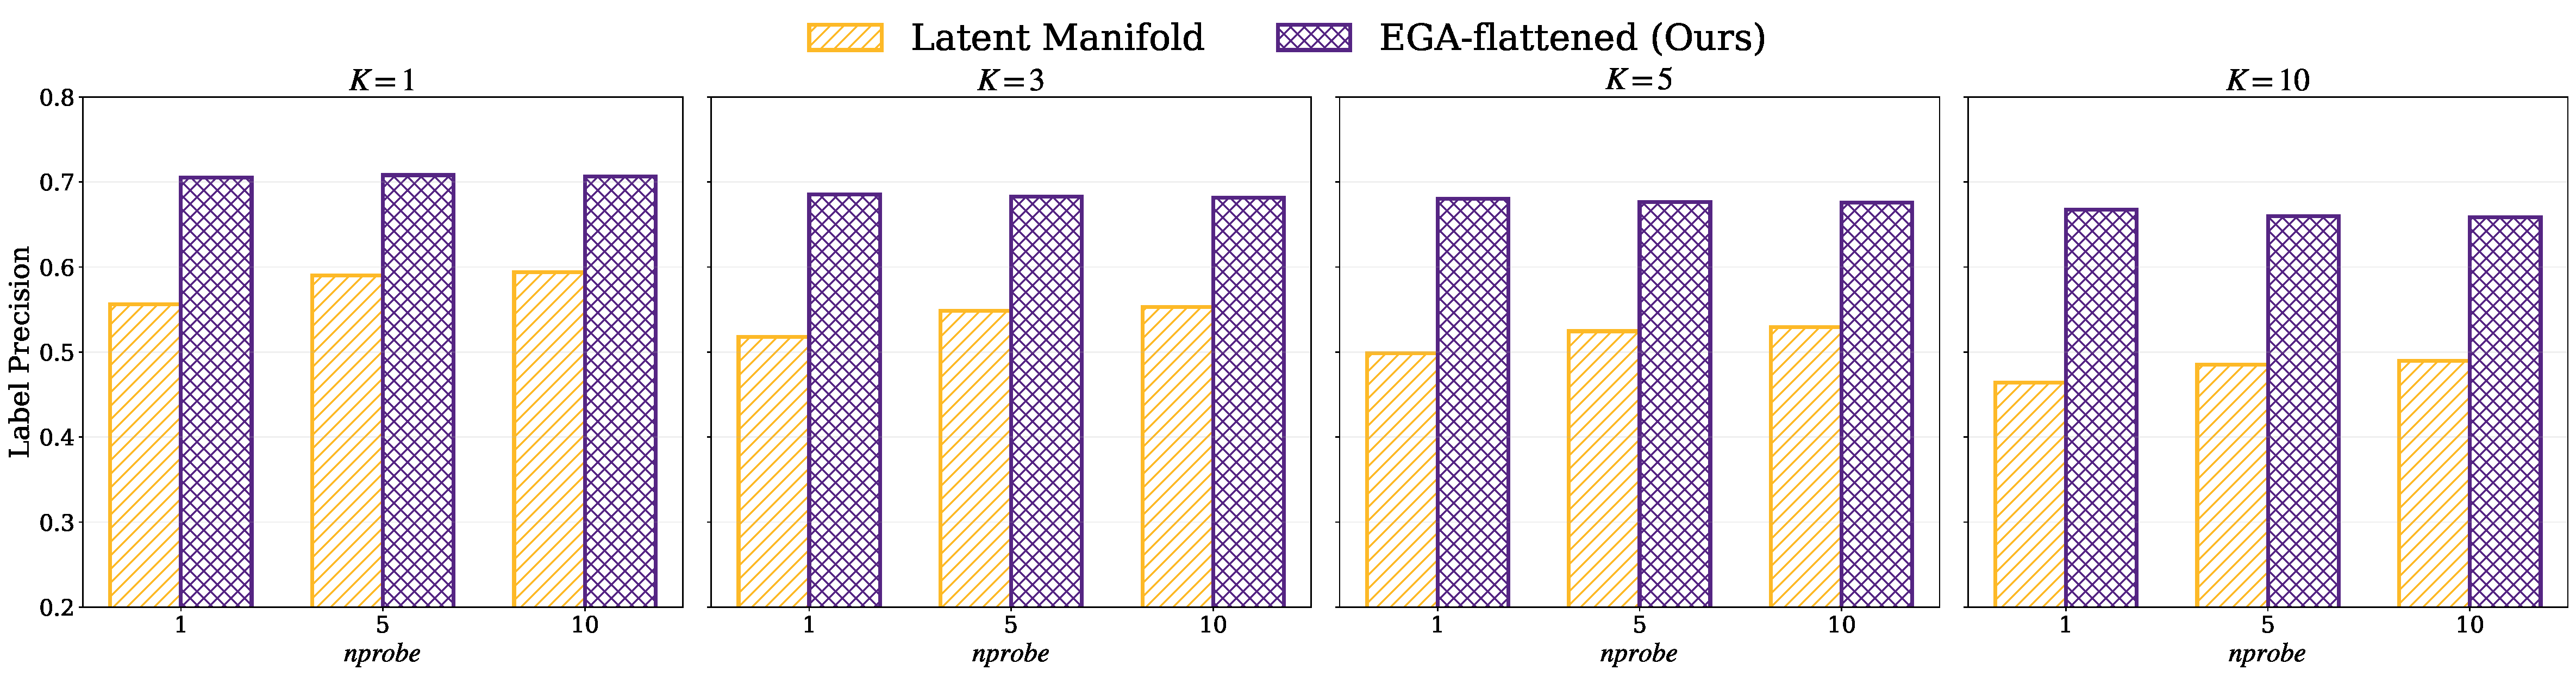
\includegraphics[width=\linewidth]{fig/label_precision.pdf}
    \caption{Label Precision@$K$ on CIFAR-100 across $K \in \{1,3,5,10\}$ and $\text{nprobe} \in \{1,5,10\}$. 
    % EGA consistently improves over the raw CLIP latent space.
    }
    \label{fig:precision_grid}
\end{figure}

\begin{figure}[t]
    \centering
    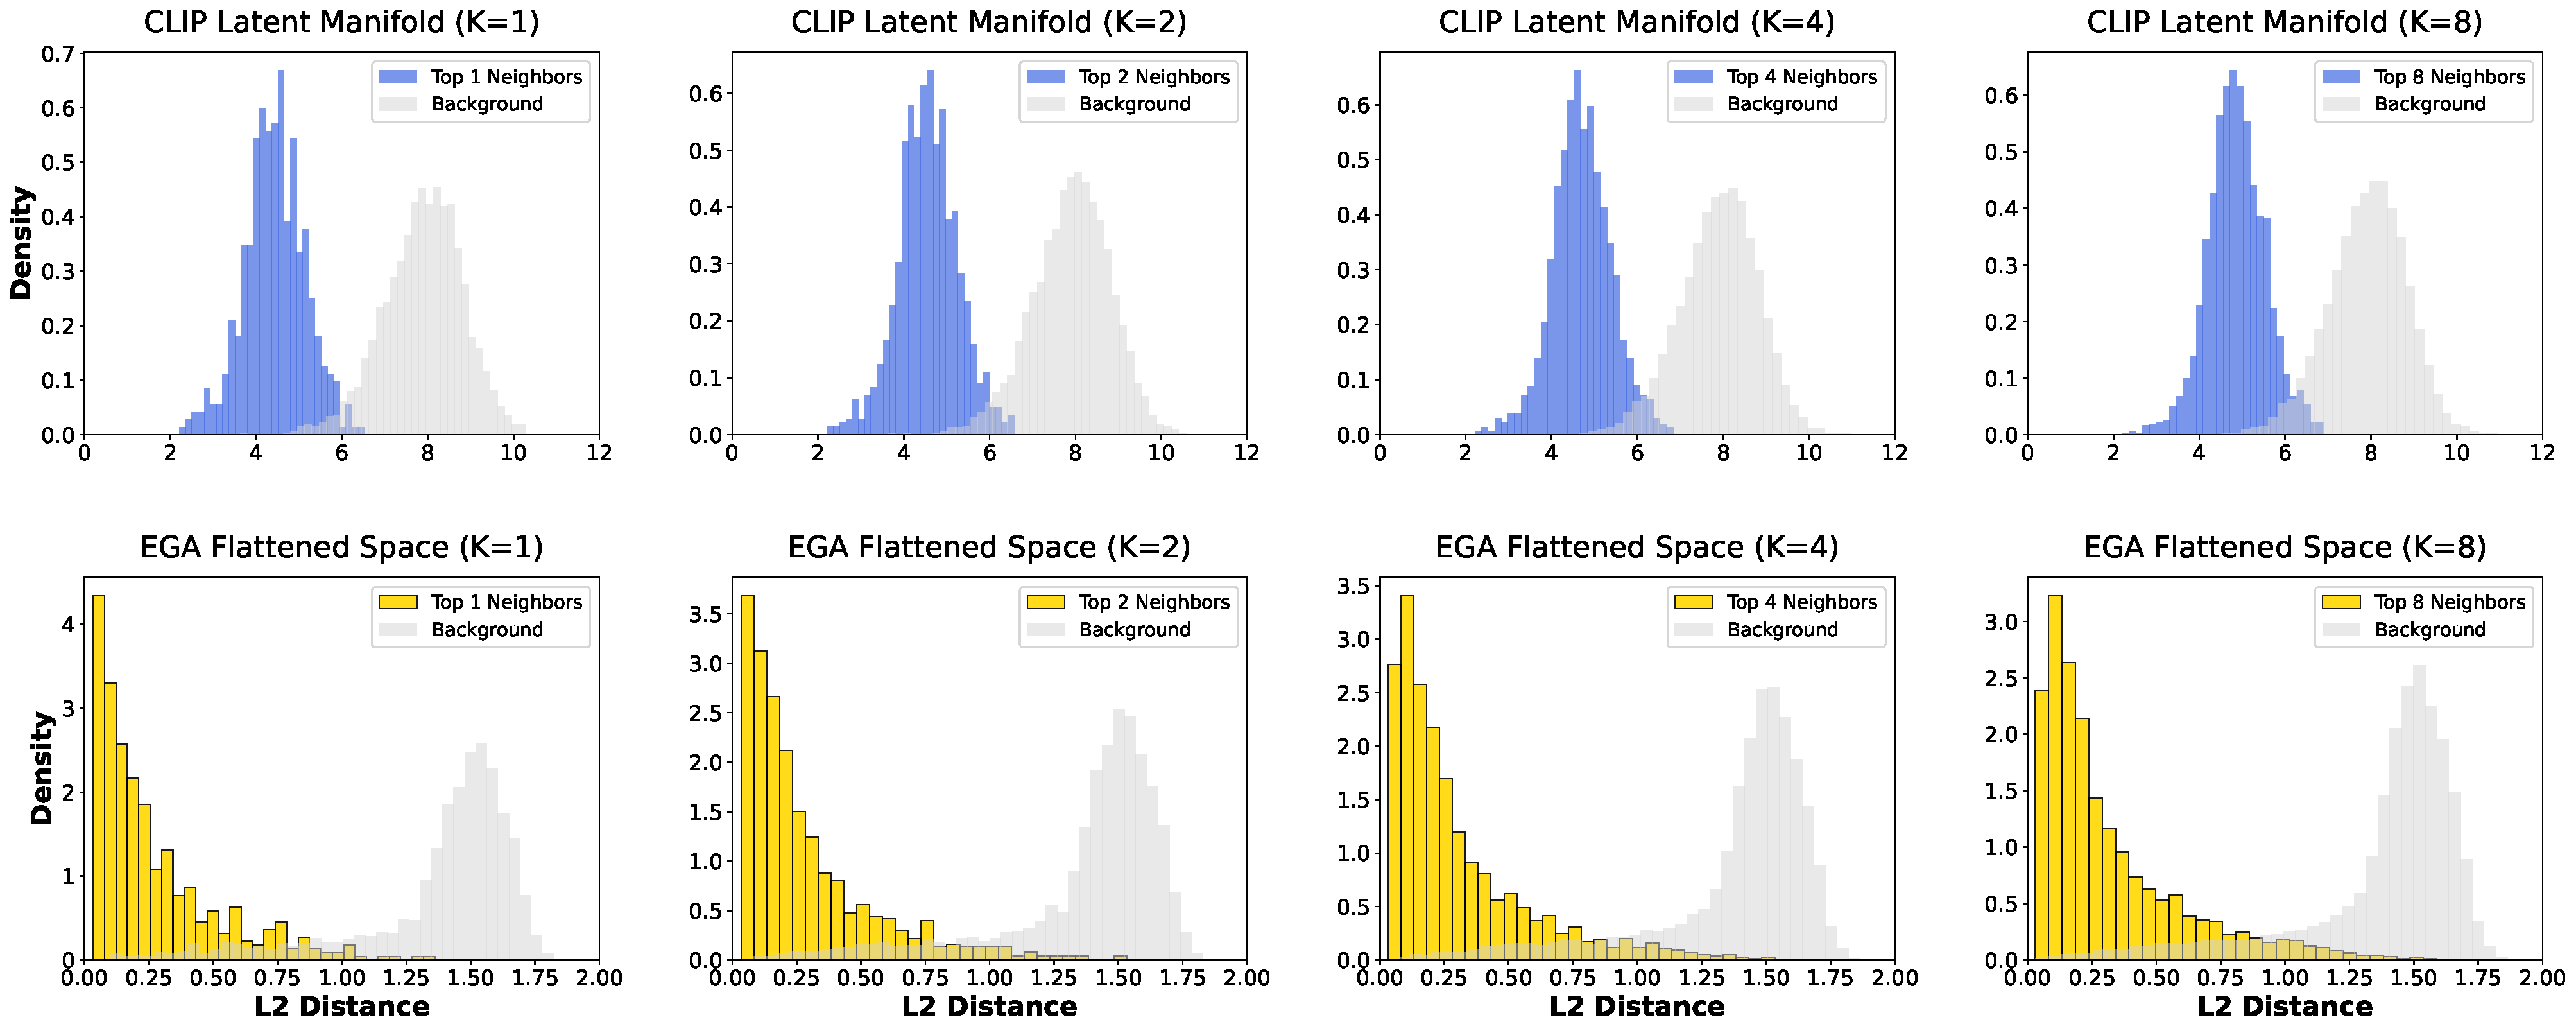
\includegraphics[width=\linewidth]{fig/distance_distribution_grid.pdf}
    \caption{$L_2$ distance distributions for Top-$K$ neighbors versus random background points on CIFAR-100. 
    % The raw CLIP space exhibits significant overlap; EGA separates the two distributions cleanly.
    }
    \label{fig:dist_grid}
\end{figure}

\begin{figure}[t]
    \centering
    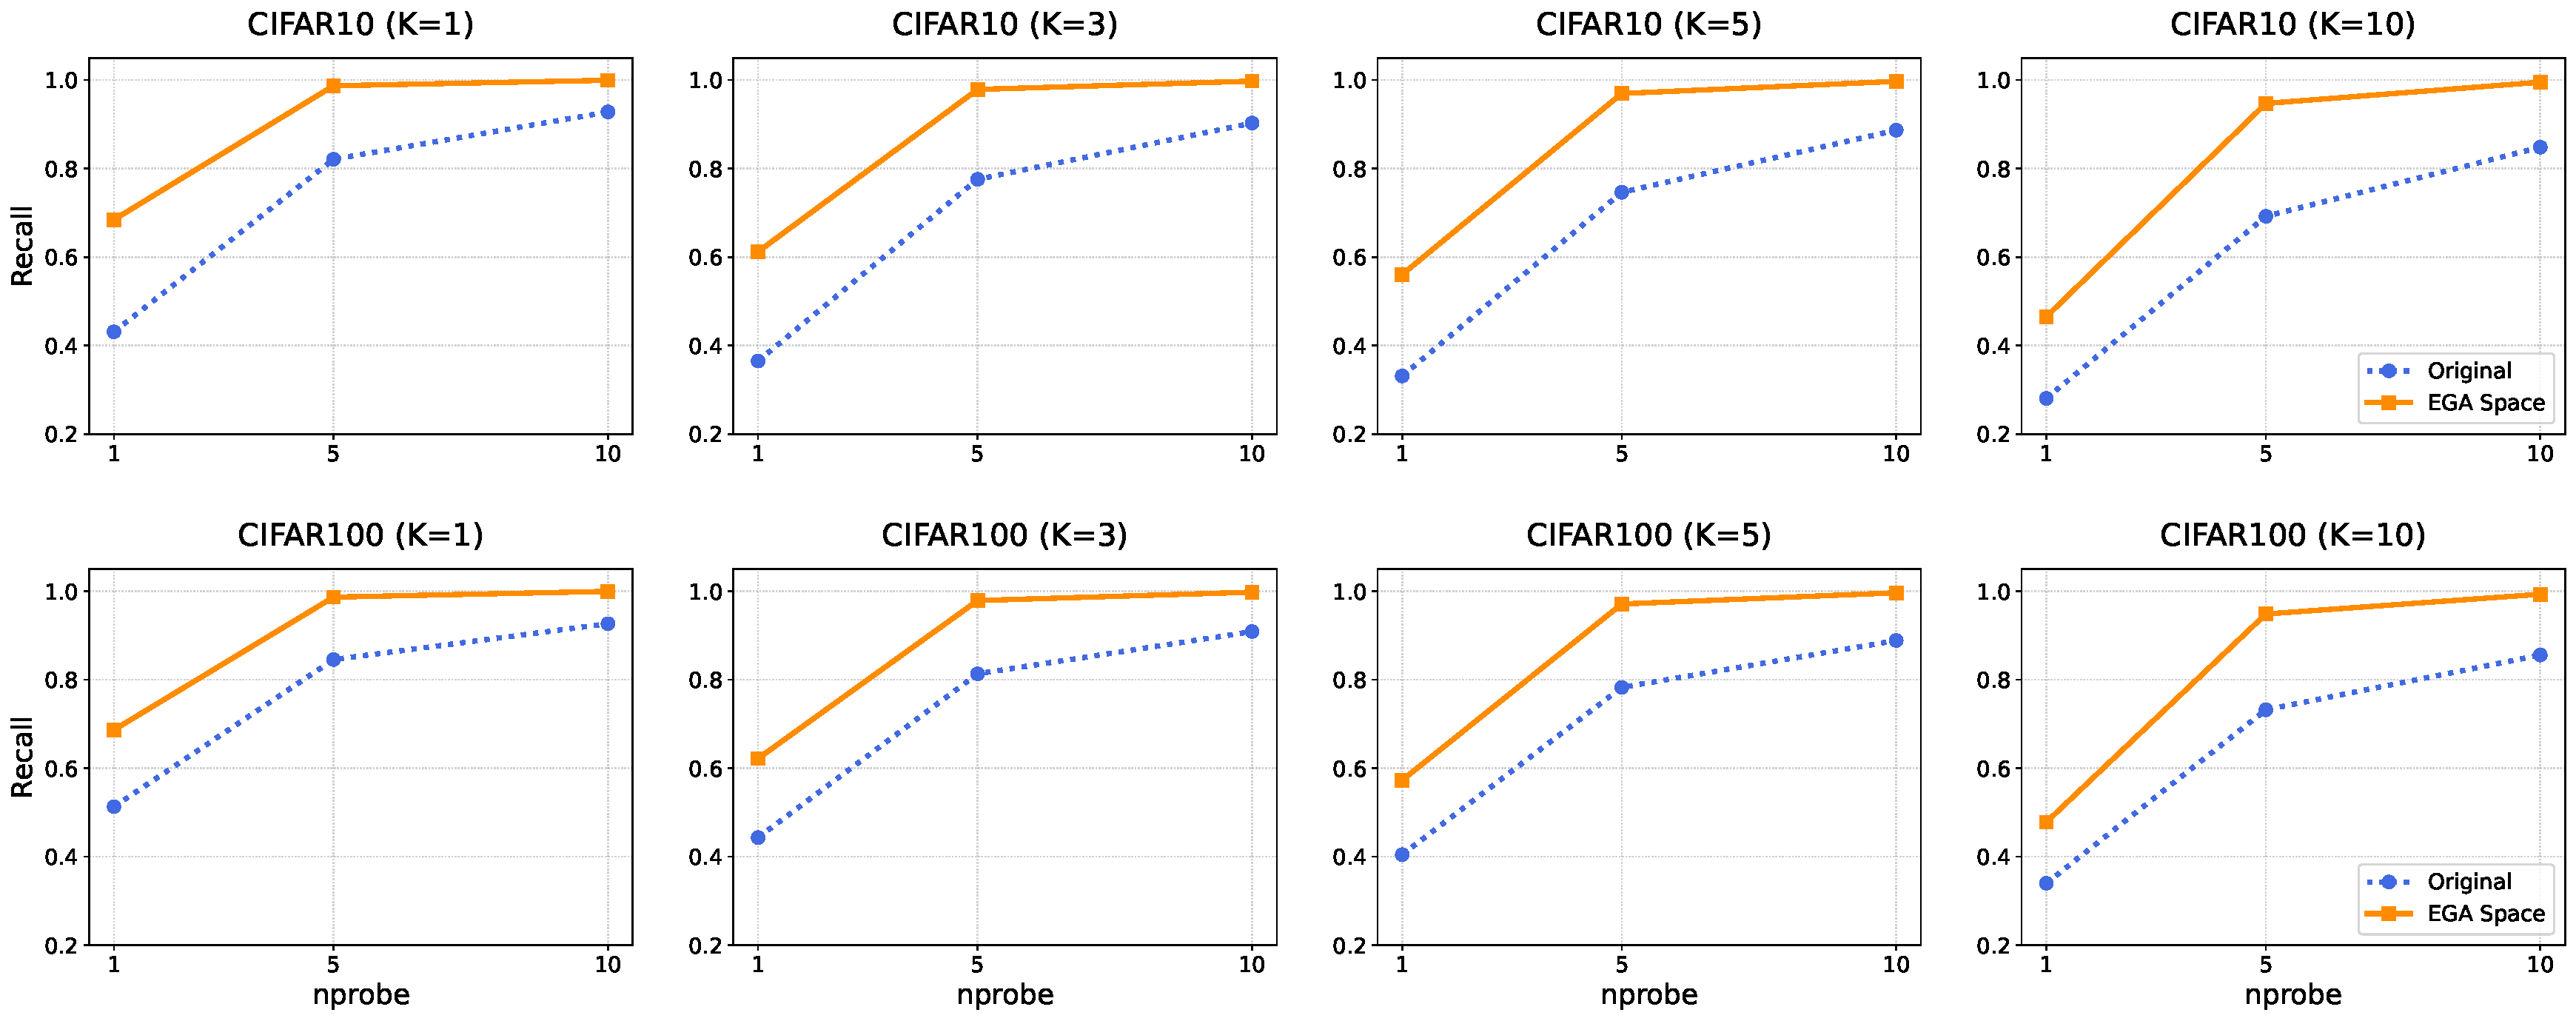
\includegraphics[width=\linewidth]{fig/recall_tradeoff_grid.pdf}
    \caption{ANNS Recall@$K$ versus $\text{nprobe}$ on CIFAR-100. 
    % EGA shifts the efficiency frontier upward across all $K$.
    }
    \label{fig:recall_grid}
\end{figure}

\paragraph{Geometric structure.}
The Label Precision improvement has a direct geometric correlate. Figure~\ref{fig:dist_grid} contrasts the $L_2$ distance distributions for true Top-$K$ neighbors against random background points, before and after EGA. In the raw CLIP space, the two distributions overlap substantially: the distance to a true neighbor is often indistinguishable from the distance to an unrelated point, which is exactly the condition under which IVF-based ANN indexing degrades. After EGA, the two distributions separate cleanly across all $K$, with neighbors concentrated at small distances and background points pushed toward a distinct mode. This separation is the mechanism by which EGA improves the recall--efficiency frontier shown in Figure~\ref{fig:recall_grid}: the raw CLIP space achieves only $0.805$ Recall@1 at $\text{nprobe}=1$, whereas EGA reaches $0.933$ and saturates above $0.97$ by $\text{nprobe}=5$.

\paragraph{In-distribution comparison across adapters.}
While Figures~\ref{fig:precision_grid}--\ref{fig:recall_grid} focus on the
EGA-vs-frozen contrast that underlies our geometric story, we also report
all six methods' in-distribution performance in
Table~\ref{tab:indist_summary}, since the contrast with their out-of-distribution
behavior (Section~\ref{sec:ood}) is central to our analysis. ICon and SRL
achieve near-perfect Label Precision ($0.999$ and $0.992$ respectively) by
maximally tightening seen-class clusters with their global contrastive
objectives. EGA reaches LP@1 of $0.700$, an improvement of $+15$ pp over the
frozen baseline; the LoRA variants land between EGA and the baseline. As we
show in Section~\ref{sec:ood}, the same property that allows ICon and SRL to
dominate this in-distribution metric is what causes their catastrophic out-of-distribution
collapse.

\begin{table}[t]
\centering
\caption{In-distribution retrieval performance on CIFAR-100 at $K=1$,
$\text{nprobe}=1$. 
% ICon and SRL dominate this metric but, as we show in
% Section~\ref{sec:ood}, fail catastrophically out-of-distribution.
}
\label{tab:indist_summary}
\small
\setlength{\tabcolsep}{4pt}
\begin{tabular}{lcccccc}
\hline
Metric & CLIP & ICon & SRL & LoRA+InfoNCE & LoRA+Triplet & EGA \\
\hline
LP@1 & 0.549 & \textbf{0.999} & 0.992 & 0.668 & 0.612 & 0.851 \\
AR@1 & 0.805 & 0.992 & 0.991 & 0.879 & 0.908 & \textbf{0.933} \\
\hline
\end{tabular}
\end{table}

\subsection{Out-of-Distribution Generalization}
\label{sec:ood}

We now turn to the central empirical claim of this paper. Under strict OOD
settings where evaluation categories are disjoint from training categories, the
two retrieval metrics tell different stories about adapter quality, and EGA is
the only method that performs well on both.
Table~\ref{tab:ood_summary} reports headline numbers at $K=1$, $\text{nprobe}=1$,
and Figure~\ref{fig:ood_lp} traces Label Precision across
$\text{nprobe} \in \{1,5,10\}$ to show that the pattern is robust to search
budget. We evaluate on three benchmarks: CIFAR-10 (trained on CIFAR-100),
FGVC-Aircraft (80 seen / 20 unseen classes), and Food-101 (80 seen / 21 unseen
classes). For a fair comparison, all methods train identical lightweight
adapters on top of frozen CLIP features and differ only in their loss functions.

\begin{table}[t]
\centering
\caption{OOD performance at $K=1$, $\text{nprobe}=1$. 
}
\label{tab:ood_summary}
\small
\setlength{\tabcolsep}{4pt}
\begin{tabular}{llcccccc}
\hline
Dataset & Metric & CLIP & ICon & SRL & LoRA+InfoNCE & LoRA+Triplet & EGA \\
\hline
\multirow{2}{*}{CIFAR-10}
  & AR@1 & 0.863 & \textbf{0.913} & \textbf{0.942} & 0.856 & \textbf{0.866} & \textbf{0.986} \\
  & LP@1 & 0.880 & \underline{0.841} & \underline{0.794} & 0.880 & \underline{0.870} & \textbf{0.886} \\
\hline
\multirow{2}{*}{Aircraft}
  & AR@1 & 0.773 & \textbf{0.875} & \textbf{0.863} & \textbf{0.911} & \textbf{0.881} & \textbf{0.898} \\
  & LP@1 & 0.512 & \underline{0.423} & \underline{0.441} & \textbf{0.560} & \textbf{0.577} & \textbf{0.548} \\
\hline
\multirow{2}{*}{Food-101}
  & AR@1 & 0.842 & \underline{0.811} & \underline{0.827} & \textbf{0.902} & \textbf{0.899} & \textbf{0.886} \\
  & LP@1 & 0.881 & \underline{0.557} & \underline{0.520} & \underline{0.878} & \underline{0.833} & \underline{0.798} \\
\hline
\end{tabular}
\end{table}

\begin{figure}[t]
    \centering
    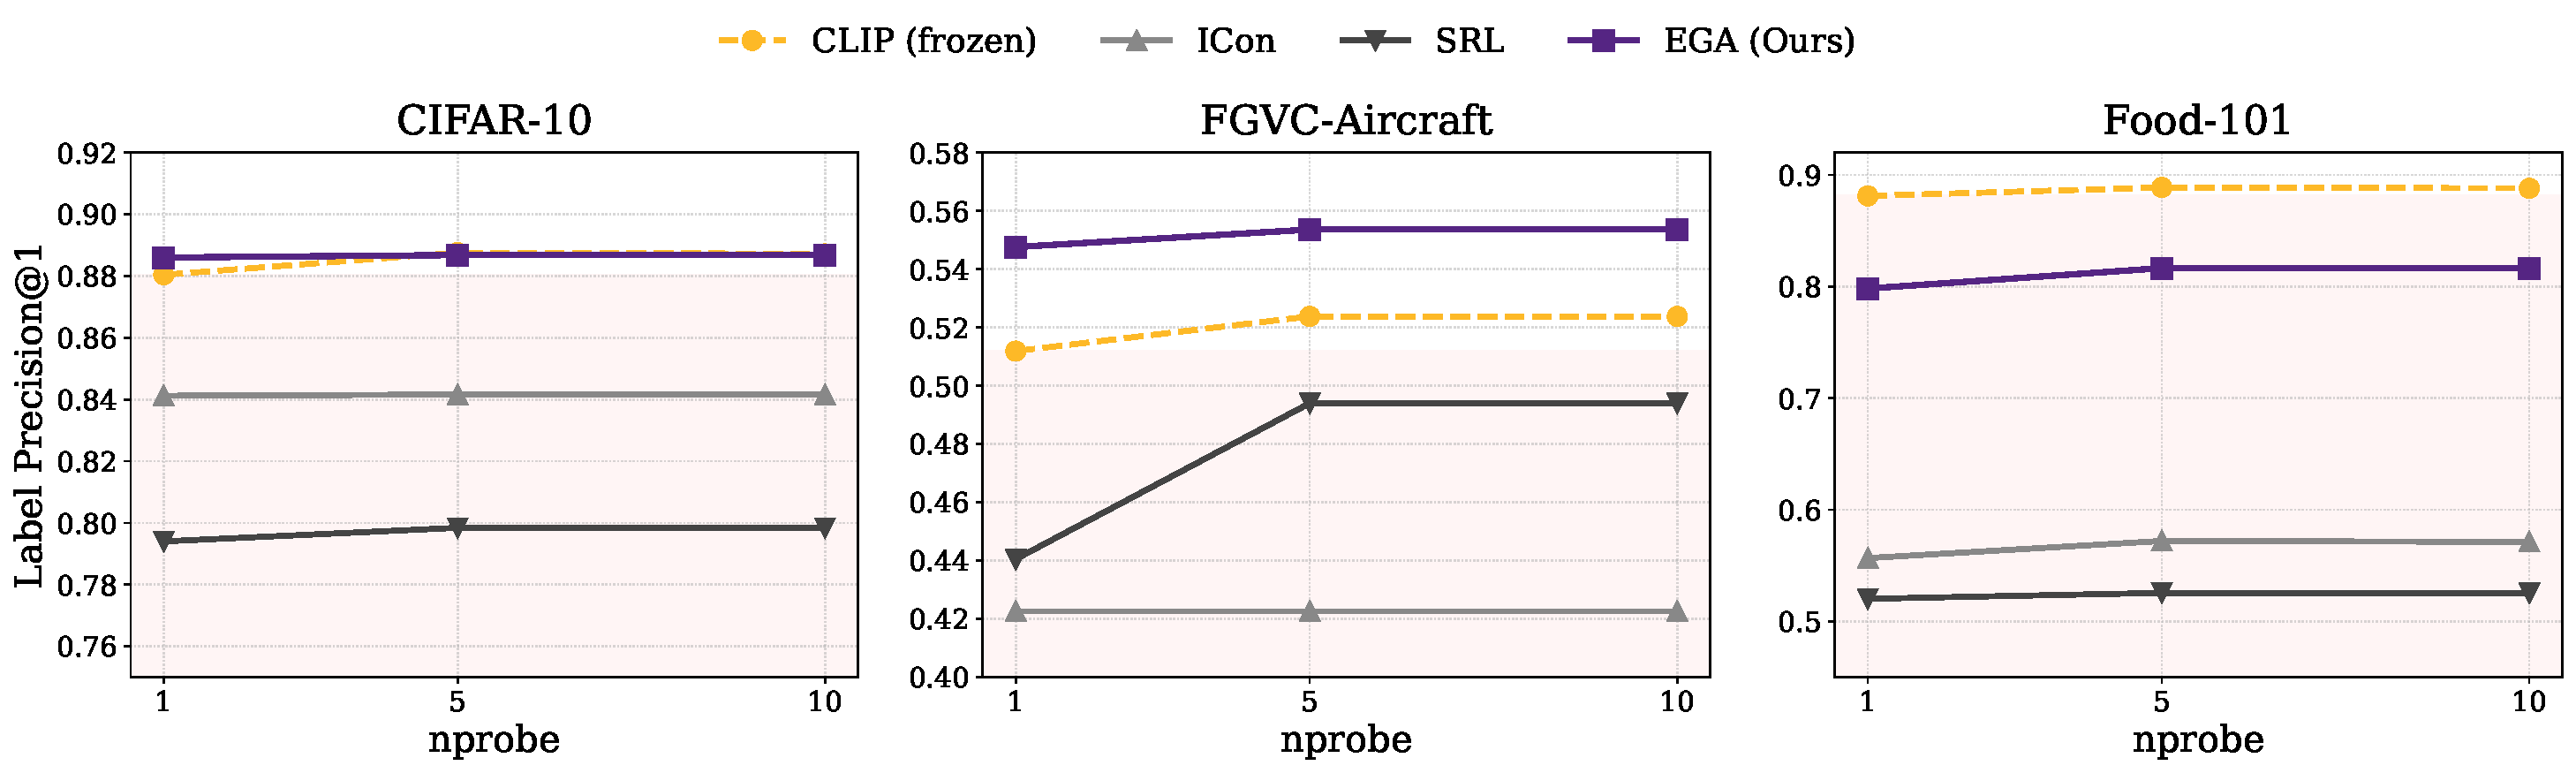
\includegraphics[width=\linewidth]{fig/ood_label_precision.pdf}
    \caption{Label Precision@1 across three OOD benchmarks and three search
    budgets. 
    }
    \label{fig:ood_lp}
\end{figure}

On ANNS Recall, every adapter improves or matches the
frozen CLIP baseline across all three OOD benchmarks (Table~\ref{tab:ood_summary}).
Adapter training succeeds at \emph{geometric} reorganization: the resulting
embedding distribution is more amenable to IVF-based indexing.
On Label Precision, however, the picture inverts. ICon and SRL fall \emph{below}
the frozen CLIP baseline on every dataset, with degradation reaching $-32$ to
$-36$ percentage points on Food-101. The retrieved neighbors are geometrically
closer in the IVF index, but they belong to the wrong semantic class. EGA is
the only adapter that improves Label Precision on Aircraft ($+3.6$ pp) and
CIFAR-10 ($+0.6$ pp), and on Food-101 it retains the strongest Label Precision
among all adapters with bounded $-8.3$ pp degradation.

The Label Precision degradation of global contrastive methods persists across
all three datasets and all three search budgets we tested ($18$ measurement points in total, Figure~\ref{fig:ood_lp}), ruling out the possibility that it
is an artifact of a particular benchmark or indexing configuration. EGA's
relative advantage over global methods ranges from $4.5$ pp on CIFAR-10 to
$24$ pp on Food-101, and tracks the difficulty of the OOD shift: when seen and
unseen classes are visually similar (as in Food-101's fine-grained dishes), the
dense gradient updates of ICon and SRL pull unseen samples most aggressively
into the wrong seen-class clusters.

Cross-referencing Table~\ref{tab:indist_summary} and
Table~\ref{tab:ood_summary} reveals a structural tradeoff among adapter
training paradigms. ICon and SRL achieve near-perfect Label Precision on
CIFAR-100 ($0.999$ and $0.992$) but collapse to $0.557$ and $0.520$ on
Food-101. The frozen baseline and LoRA variants sit at the opposite extreme:
modest in-distribution precision ($0.55$ to $0.67$) but stable performance under
distribution shift. EGA occupies a balanced position: $0.851$ in-distribution
and $0.798$ on Food-101, with $0.548$ on Aircraft and $0.886$ on CIFAR-10.
The six methods we evaluate trace out a Pareto frontier in the (ID Label
Precision, OOD Label Precision) plane, and EGA is the only adapter that is not dominated by any other: methods that exceed EGA's in-distribution
precision (ICon, SRL) collapse on OOD; methods that match or exceed EGA on OOD
(LoRA, frozen) underperform substantially in-distribution.

We evaluate LoRA~\cite{hu2022lora} as a parameter-efficient
baseline (rank $r=8$, $\sim$8K trainable parameters vs. $\sim$4.2M for the
EGAMLP architecture used by EGA, ICon, and SRL). Two configurations are
included: LoRA~+~InfoNCE (a global contrastive loss) and LoRA~+~Triplet (the
same loss as EGA). Both LoRA configurations avoid the Label
Precision collapse exhibited by ICon and SRL even when paired with a global
loss: LoRA~+~InfoNCE on Food-101 reaches LP $0.878$, only $0.3$ pp below the
frozen baseline. This suggests that the failure of ICon and SRL
arises from the \emph{combination} of (i) full-capacity adapter and (ii) dense
global gradients, not from the global loss alone. With an aggressive bottleneck
on adapter capacity, global losses become survivable. 

\subsection{Gradient Sparsity as OOD Protection}
\label{sec:mechanism}

The OOD pattern in Section~\ref{sec:ood} raises a mechanistic question: why does EGA's triplet objective preserve unseen-class structure while global contrastive objectives reshape it? We identify gradient sparsity at convergence as the key mechanism.

A triplet loss with margin $m$ produces a non-zero gradient for a sample triplet
$(a, p, n)$ only when the margin constraint is violated, i.e., when
\begin{equation}
    d(a, p) - d(a, n) + m > 0.
    \label{eq:active_triplet}
\end{equation}
As the adapter converges on seen classes, the fraction of \emph{active}
triplets decays. Figure~\ref{fig:mechanism} (left) tracks this ratio
throughout training: starting at $17.4\%$ at epoch~10, it falls to $3.5\%$ by
convergence. At steady state, 96.5\% of triplets contribute zero
gradient, meaning the adapter updates a sparse subset of local neighborhood
relationships and leaves the remainder of the embedding space intact.

Global contrastive objectives such as ICon~\cite{alshammariunifying} and SRL~\cite{dong2025improve} exhibit
the opposite behavior. ICon minimizes a KL divergence over the full pairwise
similarity matrix, and SRL jointly optimizes batch-wide uniformity and
homogeneity. Both produce \emph{dense} gradient fields in every training step:
every sample pair contributes to the loss regardless of whether its local geometry
already satisfies the retrieval objective. This global optimization pressure shapes the entire embedding distribution
based on seen-class similarities, even for regions of the space occupied by
unseen-class samples. The result is not loss of geometric structure but rather
loss of \emph{semantically correct} structure: unseen samples are pulled
toward the clusters of seen classes that they happen to resemble in CLIP's
original metric, rather than toward other unseen samples that share their
true category.

\begin{wrapfigure}{r}{0.52\textwidth}
% \vspace{-1em}
\centering
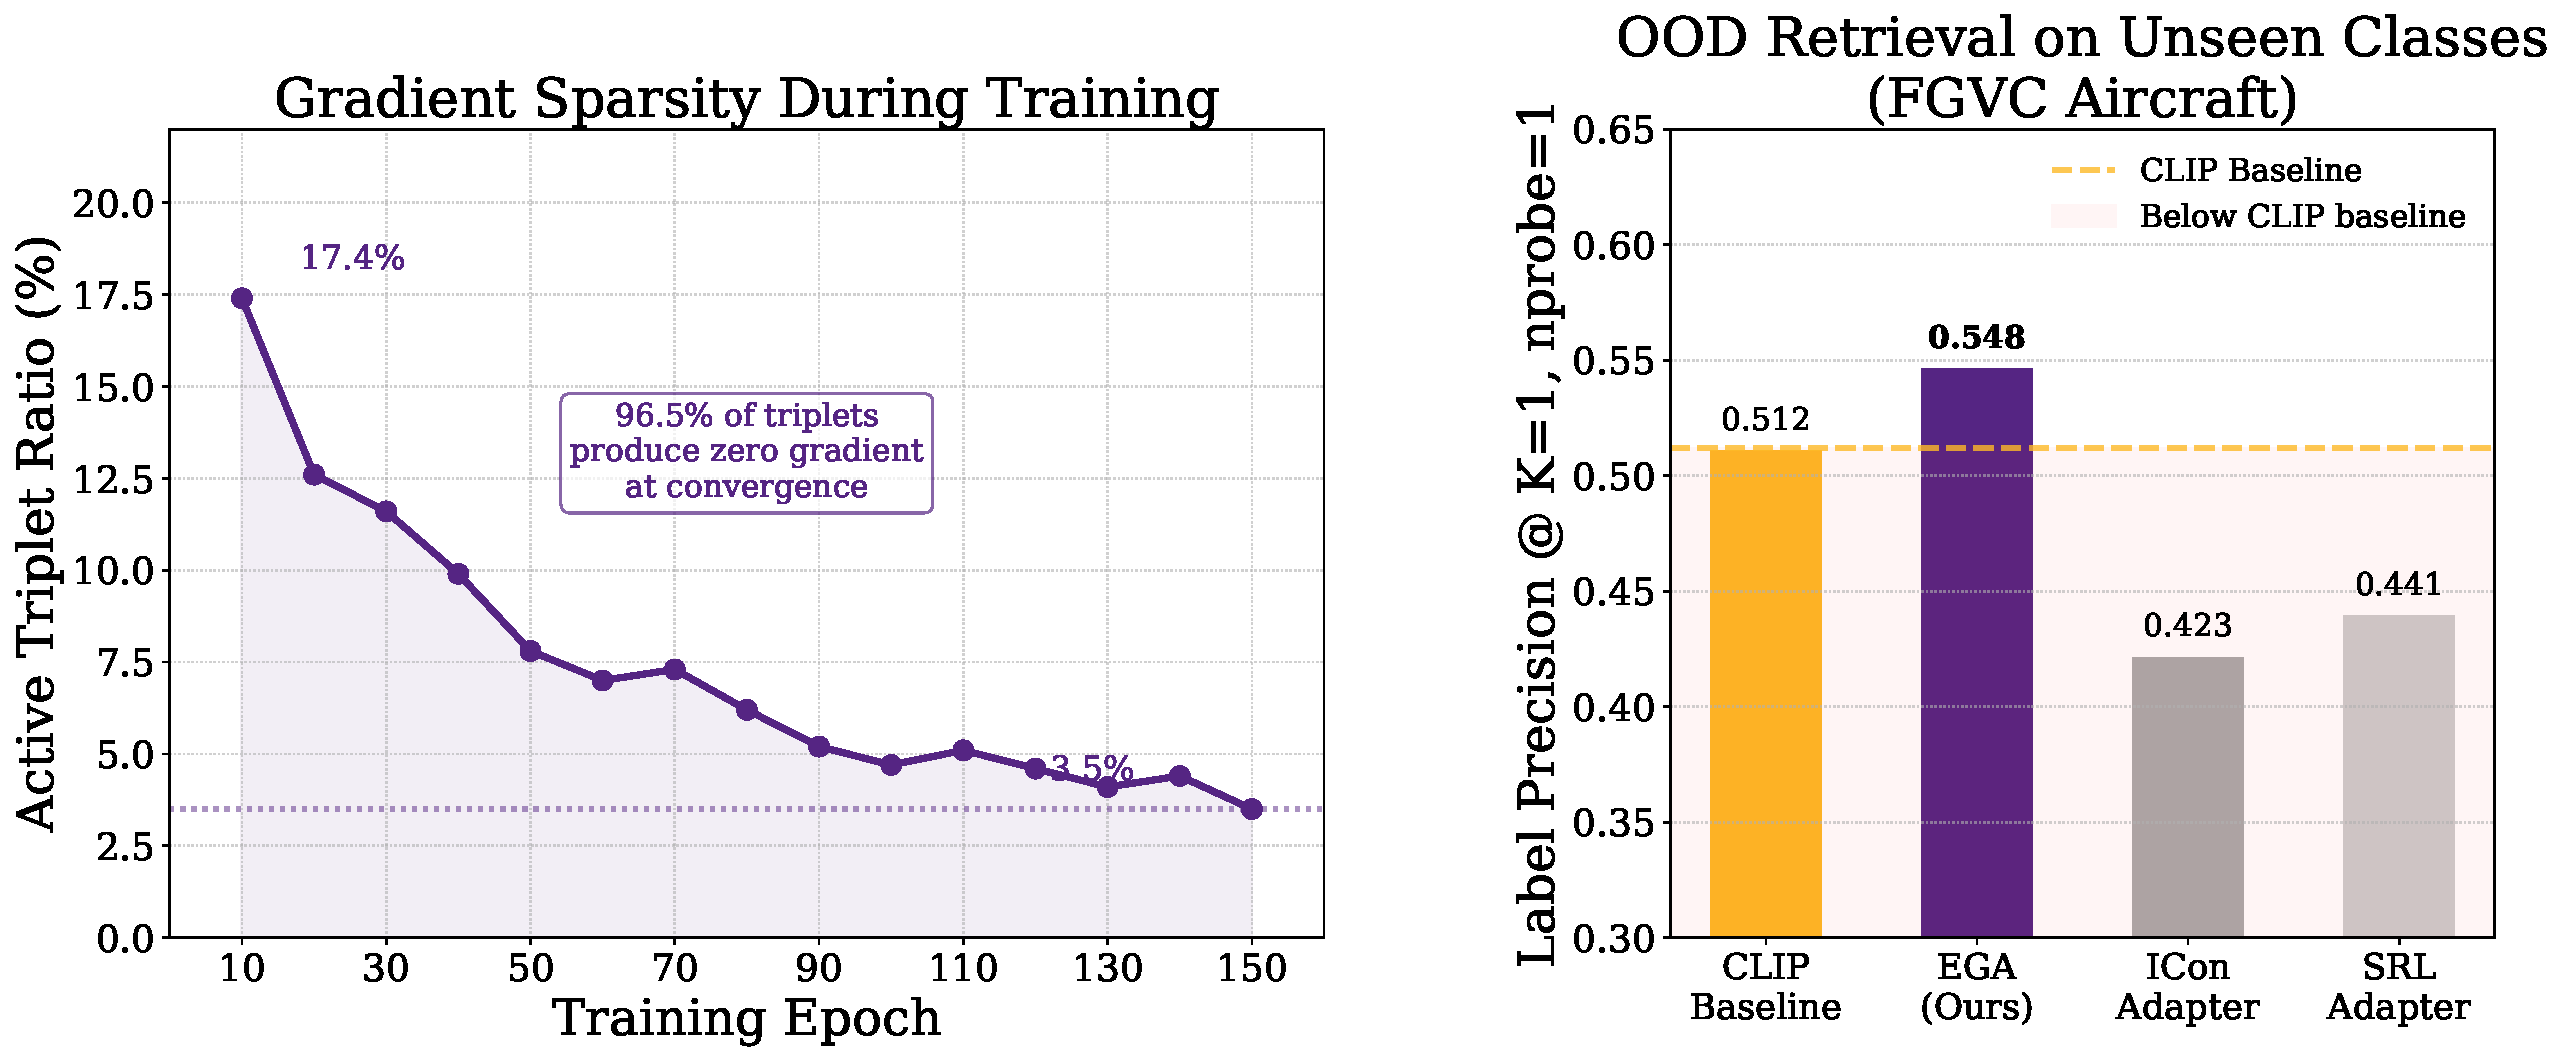
\includegraphics[width=0.98\linewidth]{fig/mechanism_sparse_gradient.pdf}
\caption{Gradient sparsity as OOD protection.
}
\label{fig:mechanism}
% \vspace{-1em}
\end{wrapfigure}
Figure~\ref{fig:mechanism} (right) and Figure~\ref{fig:ood_lp} together
quantify the consequence: across all three OOD benchmarks, ICon and SRL fall
below the frozen CLIP baseline on Label Precision (e.g., on Aircraft, ICon
collapses to $0.423$ from a baseline of $0.512$), confirming that dense gradient
updates actively harm zero-shot semantic retrieval. 
EGA, by contrast, improves Label Precision on Aircraft and CIFAR-10 while only $3.5\%$ of training triplets contribute non-zero gradients at convergence.

\subsection{Ablation and Sensitivity Analysis}
\label{sec:ablation}

\begin{table}[t]
\centering
\begin{minipage}{0.38\textwidth}
\centering
\caption{Ablation study of EGA}
\label{tab:ablation}
\small
\begin{tabular}{lc}
\hline
Variant & Accuracy \\ \hline
Full EGA (Ours) & 0.7015 \\
w/o Residual connection & 0.0065 \\
w/o Zero-initialization & 0.6840 \\
w/o L2-normalization & 0.6590 \\ \hline
\end{tabular}
\end{minipage}
\hfill
\begin{minipage}{0.61\textwidth}
\centering
\caption{Sensitivity of different hyperparameters}
\label{tab:sensitivity}
\small
\begin{tabular}{lcccc}
\hline
Triplet Margin $m$ & 0.1 & 0.2 & 0.3 & 0.5 \\ \hline
Recall@1 & 0.8420 & 0.8180 & 0.8160 & 0.7400 \\
Recall@5 & 0.9782 & 0.9654 & 0.9610 & 0.9125 \\ \hline
Hidden Dimension $d$ & 512 & 1024 & 2048 & 4096 \\ \hline
Recall@1 & 0.8300 & 0.8340 & 0.8200 & 0.8240 \\
Recall@5 & 0.9695 & 0.9712 & 0.9680 & 0.9688 \\ \hline
\end{tabular}
\end{minipage}
\end{table}

Table~\ref{tab:ablation} isolates the contribution of each architectural component. The residual connection is the core element. Removing it causes accuracy to collapse from 0.7015 to 0.0065. This collapse indicates that the adapter cannot reconstruct semantic relationships from target data alone and must operate as a refinement over the pre-trained features. The L2 normalization ensures the transformed embeddings remain on the unit hypersphere. Removing this constraint decreases accuracy to 0.6590. Zero-initialization allows the adapter to begin training as an identity mapping. Removing it lowers accuracy to 0.6840.

Table~\ref{tab:sensitivity} evaluates model stability across hyperparameter variations. EGA maintains consistent retrieval quality across margin values from 0.1 to 0.3. Increasing the margin to 0.5 degrades Recall@1 to 0.7400. A larger margin forces the adapter to update embeddings that already satisfy local neighborhood constraints, which reduces gradient sparsity and alters the pre-trained manifold. Furthermore, the model shows stable performance across hidden dimensions ranging from 512 to 4096. This stability confirms that EGA achieves metric correction through its structural design rather than specific parameter capacities.

\section{Conclusion}
\label{sec:conclusion}

We have shown that lightweight adapter training over frozen CLIP does not produce uniformly improved retrieval embeddings, but instead lands different methods at different points along an in-distribution/out-of-distribution Pareto frontier. High-capacity adapters trained with global contrastive objectives (ICon, SRL) reach near-perfect Label Precision on CIFAR-100 ($0.999$, $0.992$) but collapse below the frozen baseline by $32$ to $36$ percentage points on Food-101. Low-capacity LoRA adapters avoid this collapse but underperform substantially in-distribution. EGA, our proposed manifold-preserving adapter, occupies a balanced Pareto-optimal position: it reaches $0.851$ in-distribution Label Precision while improving over the frozen baseline on two of three OOD benchmarks and bounding the degradation on the third. The mechanism is gradient sparsity at convergence, i.e., $96.5\%$ of training triplets produce zero gradient at steady state, which permits high-capacity in-distribution refinement while leaving most of the embedding space, including regions occupied by unseen categories, largely unmodified.

% The broader observation is that adapter design choices for foundation-model retrieval should be evaluated on the joint (ID, OOD) frontier rather than on either axis in isolation. Methods that compress seen-class clusters most aggressively are not necessarily the methods that generalize best, and methods that generalize best are not necessarily the methods that refine seen classes most precisely. Gradient sparsity at convergence is a measurable training-time property that predicts where an adapter will land on this frontier, and we suggest it as a useful diagnostic for future adapter design.

\paragraph{Limitations.}
This study focuses on visual representations from CLIP. Future work will extend EGA to text and multimodal models, explore unsupervised variants, and more rigorously disentangle the joint role of adapter capacity and loss sparsity in shaping the ID/OOD Pareto frontier.

\bibliography{ref}
\bibliographystyle{plain}

\clearpage
\input{checklist.tex}

\clearpage
\appendix

\section{Proof of Proposition~\ref{prop:sparsity}}
\label{proof:sparsity}
 
\begin{proof}
We prove each claim in turn.
 
\textbf{(1) Gradient support.}
The triplet loss in Eq.~\eqref{eq:triplet} can be written as
$\mathcal{L} = \frac{1}{|\mathcal{B}|}\sum_{(a,p,n)\in\mathcal{B}} \ell_{apn}$,
where $\ell_{apn} = \max(0, \delta_{apn} + m)$ and
$\delta_{apn} = d(\hat{\mathbf{z}}_a, \hat{\mathbf{z}}_p)
              - d(\hat{\mathbf{z}}_a, \hat{\mathbf{z}}_n)$.
The subgradient with respect to $\theta$ is
\begin{equation}
    \nabla_\theta \ell_{apn} =
    \mathbf{1}[\delta_{apn} + m > 0]\cdot
    \nabla_\theta \delta_{apn},
\end{equation}
which is exactly zero whenever $\delta_{apn} + m \leq 0$. Therefore,
$\nabla_\theta \mathcal{L}$ receives contributions only from active
triplets satisfying Eq.~\eqref{eq:active}.
 
\textbf{(2) Convergence of $\rho(t)$.}
Under mild regularity conditions (Lipschitz continuity of $f_\theta$ and
bounded embedding norms), the sequence $\{\hat{\mathbf{z}}^{(t)}\}$ converges
to a stationary point $\hat{\mathbf{z}}^*$ of $\mathcal{L}$. At stationarity,
$\rho(t)$ converges to $\rho^*$ as defined in Eq.~\eqref{eq:rho_star},
since $\rho(t)$ is a continuous functional of the embedding distribution and
the embeddings converge.
 
\textbf{(3) Empirical locality (conjecture).}
Strictly speaking, parameter updates $\nabla_\theta \delta_{apn}$ computed on
seen-class triplets affect $f_\theta$ globally (including its behavior on
unseen-class inputs) since $f_\theta$ is a parametric MLP and is not
locally supported on the input manifold. We therefore do not claim formal
zero-gradient over unseen regions. Instead, we conjecture an
\emph{empirical} locality property: when (i) the residual structure with
zero initialization keeps the cumulative perturbation magnitude bounded by
the sum of training gradients, and (ii) gradient sparsity at convergence
($\rho^* \approx 3.5\%$ on FGVC-Aircraft) attenuates this sum, the resulting
perturbation in unseen-class regions is small enough to preserve the
pretrained semantic structure for retrieval purposes. This conjecture is
empirically supported by the OOD Label Precision results in
Section~\ref{sec:ood} and Figure~\ref{fig:ood_lp}, where EGA preserves or
improves Label Precision on unseen categories while ICon and SRL, which
lack the gradient sparsity property, collapse below the frozen baseline.
A formal Lipschitz-based bound on this perturbation is left for future work.
 
\textbf{(4) Dependence on $m$.}
The residual distance gap $\delta^*_{apn}$ at convergence is bounded by the
within-class diameter $\Delta_c = \max_{x,x' \in c} d(\hat{\mathbf{z}},
\hat{\mathbf{z}}')$ for seen class $c$. For $m \leq \min_c \Delta_c$,
the adapter can drive all within-class distances below the threshold, pushing
$\rho^*$ toward zero. For $m > \min_c \Delta_c$, some triplets remain
active at convergence because the within-class spread exceeds the margin,
resulting in a strictly positive $\rho^*$. This explains the empirically
observed increase in $\rho^*$ with larger $m$ reported in
Table~\ref{tab:sensitivity}.
\end{proof}
 
\section{More Experimental Details}
\label{sec:more_experiments}

\paragraph{Datasets.}
We evaluate on four datasets covering both in-distribution and OOD retrieval
scenarios. \textbf{CIFAR-100}~(100 classes, 60K images) serves as the
in-distribution benchmark: the adapter is trained and evaluated on the same
class label space, with a 75/25 split between database and query sets.
\textbf{CIFAR-10}~(10 classes, 60K images) provides a cross-dataset OOD setting:
the adapter is trained on CIFAR-100 and evaluated on the disjoint CIFAR-10
classes. \textbf{FGVC-Aircraft}~(100 fine-grained aircraft variants, 10K images)
and \textbf{Food-101}~(101 food categories, 25K images for the test split we
use) provide unseen-class OOD settings: classes are randomly partitioned into
$80\%$ seen / $20\%$ unseen with a fixed seed, the adapter is trained on the
seen split, and retrieval is evaluated strictly on the unseen split. Image
embeddings for all datasets are extracted with frozen CLIP ViT-B/32.

\paragraph{Baselines.}
We compare EGA against the frozen CLIP baseline and four trained adapters,
all sharing the same training data, evaluation protocol, and 75/25 retrieval
split:
\begin{itemize}
    \item \textbf{ICon}~\cite{alshammariunifying}: a global contrastive
    objective minimizing the KL divergence between the empirical similarity
    distribution and the class-membership distribution. We instantiate ICon on
    the same EGAMLP architecture used by our method ($\sim$4.2M parameters).
    \item \textbf{SRL}~\cite{dong2025improve}: a structural regularization
    objective jointly optimizing batch-wide uniformity and within-class
    homogeneity, also instantiated on the EGAMLP architecture.
    \item \textbf{LoRA~+~InfoNCE}~\cite{hu2022lora,oord2018representation}: a low-rank adapter (rank $r=8$,
    $\alpha=16$, $\sim$8K parameters) with zero-initialized residual structure,
    trained with supervised InfoNCE, which is a standard global contrastive loss.
    \item \textbf{LoRA~+~Triplet}~\cite{hu2022lora}: identical low-rank architecture as above,
    but trained with the same small-margin ($m=0.2$) triplet loss as EGA.
\end{itemize}
The two LoRA configurations isolate the effect of architectural capacity vs.
loss function: comparing LoRA~+~InfoNCE against ICon/SRL holds the loss family
roughly fixed while changing capacity, and comparing LoRA~+~Triplet against
EGA holds the loss fixed while changing capacity.

\paragraph{Indexing and metrics.}
For all retrieval evaluations we use FAISS~\cite{johnson2019billion}
\texttt{IndexIVFFlat} with $\text{nlist}{=}10$ centroids and report results at
$\text{nprobe} \in \{1, 5, 10\}$. We measure both Label Precision~(LP@$K$,
Eq.~\ref{eq:lp}) and ANNS Recall~(AR@$K$, Eq.~\ref{eq:ar}) at
$K \in \{1, 3, 5, 10\}$.

\paragraph{Training.}
All adapters are trained for 150 epochs with AdamW (weight decay $10^{-4}$),
cosine-annealed learning rate, and batch size 256. EGAMLP-based methods (EGA,
ICon, SRL) use learning rate $10^{-4}$; LoRA variants use $10^{-3}$ to compensate
for their smaller parameter count. Triplet-based methods sample one positive and
one negative per anchor uniformly within each mini-batch; global contrastive
methods (ICon, SRL, LoRA~+~InfoNCE) operate on the full pairwise similarity
matrix. All experiments use a fixed random seed (42) for reproducibility.

\paragraph{Compute platform.}
All experiments were conducted on the Chameleon Cloud~\cite{keahey2020lessons}
platform using a compute node equipped with 256 AMD EPYC-7763 CPU cores,
512 GiB of RAM, and an NVIDIA A100 GPU of 80 GB HBM2e. The operating system is
Ubuntu 24.04 LTS.

\end{document}